\label{app:chap3}

This appendix shows supportive information and figures that belong to Chapter \ref{chap3}.



\section{Mesh refinement analysis}

Proper meshing is crucial in order to obtain accurate simulation data. Coarse meshes will generally result in poor results badly representation of the actual deformation of a system. Fine meshes will consume a lot or RAM and therefore take up a lot of computation time. Therefore, a valid mesh size needs to be obtained, which balances accuracy of output data and computation time. To this end, multiple simulations are carried out in $\verb+Abaqus/CAE+$ to justify the mesh size.

In the simulation both bellows are pressurized to $80$ kPa, which is the theoretical maximum of the air pumps on the physical system. Multiple simulation will be carried out for an increased amount of nodes. These nodes are a measure for the mesh-size. The length difference between the undeformed top plate and deformed top plate will be calculated for each simulation. This length difference will be addressed as elongation. Figure \ref{fig3:meshrefinement} shows the determined elongation as a function of amount of nodes.

\begin{figure}[H]
    \centering
    \includegraphics[width = 0.8\textwidth]{Figures/Chapter2/MeshRefinement.eps}
    \caption{Mesh refinement analysis for a bellow pressure of $80$kPa.}
    \label{fig3:meshrefinement}
\end{figure}


Figure (\ref{fig3:meshrefinement}) shows that from 60 thousand nodes onwards the elongation data may be deemed reliable. A lower amount of nodes results in poor data output. It can also be seen that increasing the amount of nodes does not improve the simulation output any further. At 60 thousand nodes, the elongation has already converged.
